\documentclass[a4paper]{scrreprt}
\setcounter{tocdepth}{3}
\setcounter{secnumdepth}{3}

\usepackage[german]{babel}
\usepackage[utf8]{inputenc}
\usepackage[T1]{fontenc}
\usepackage{ae}
\usepackage{graphicx}


\begin{document}
\title{Entwurf}
\author{Fangzhou Bian, Kathrin Blum, Matthias Bruns, \\Leonhard Duda, Tan Grumser, Yuguang Lin}
\maketitle
%\Footnote für Fußnoten
% Platzierung des Inhaltsverzeichnisses
\tableofcontents



\chapter{Einleitung}

\chapter{Grobentwurf}
\section{Systemarchitektur}
\section{Systemkomponenten}
\section{Komponentenbeschreibung}
\subsection{Client}
\subsection{Server}


\chapter{Feinentwurf}
\section{Klassen des Clients}
\subsection{Klassendiagramm}
\subsubsection{Muster}

\section{Klassen des Server}
\subsection{Klassendiagramm}
\subsubsection{Muster}


\chapter{Datenstrukturen}

\chapter{Dynamische Modelle}
\section{Aktivitätsdiagramm}

\section{Sequenzdiagramm}
\subsection{Registrieren}
\begin{center}
	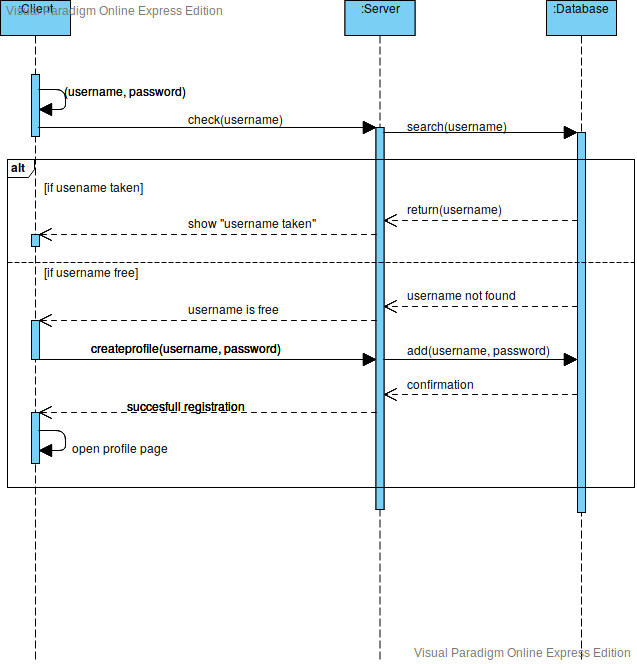
\includegraphics[width=0.93\textwidth]{Sequenzdiagramme/SequenzdiagramRegistration.jpg}
\end{center}

\subsection{Mensalinien wählen}
\begin{center}
	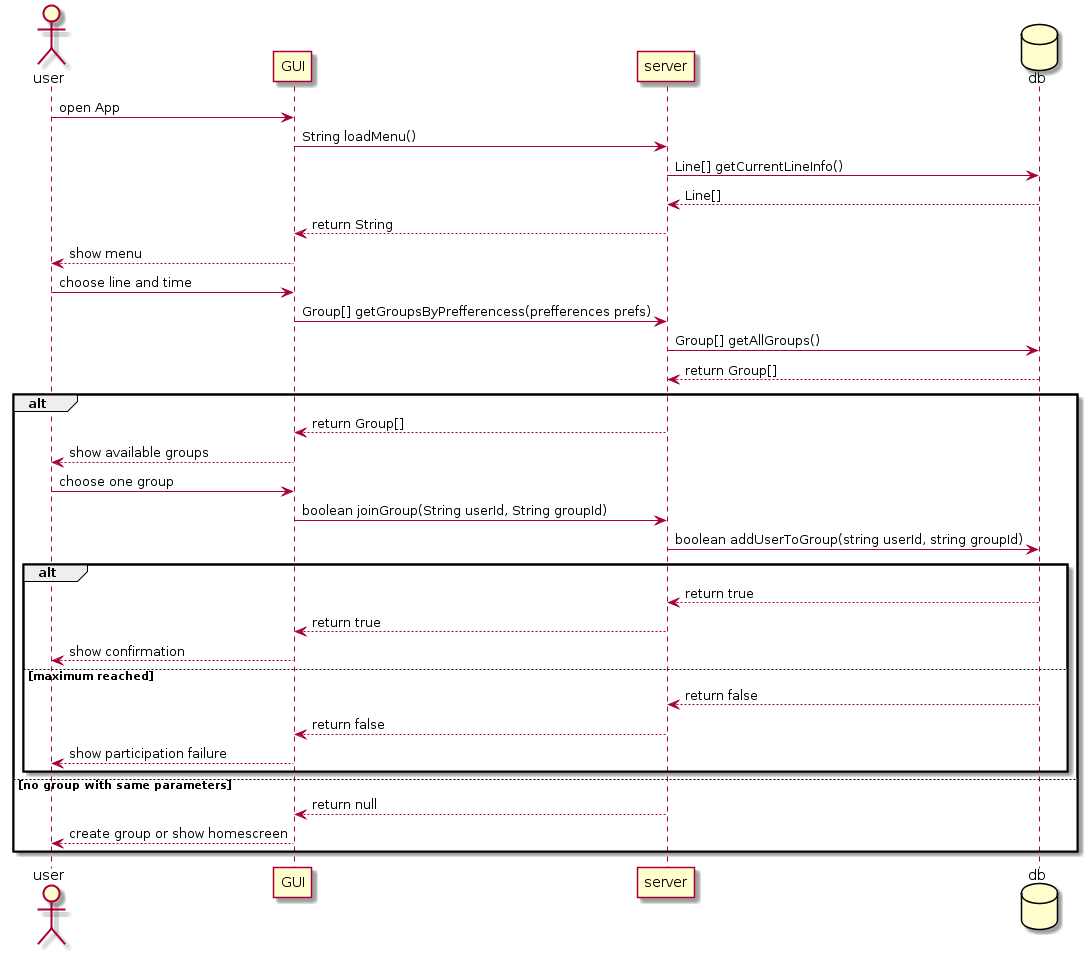
\includegraphics[width=0.93\textwidth]{Sequenzdiagramme/chooseLineAndTimeSD.png}
\end{center}


\subsection{Gruppe beitreten}
\begin{center}
	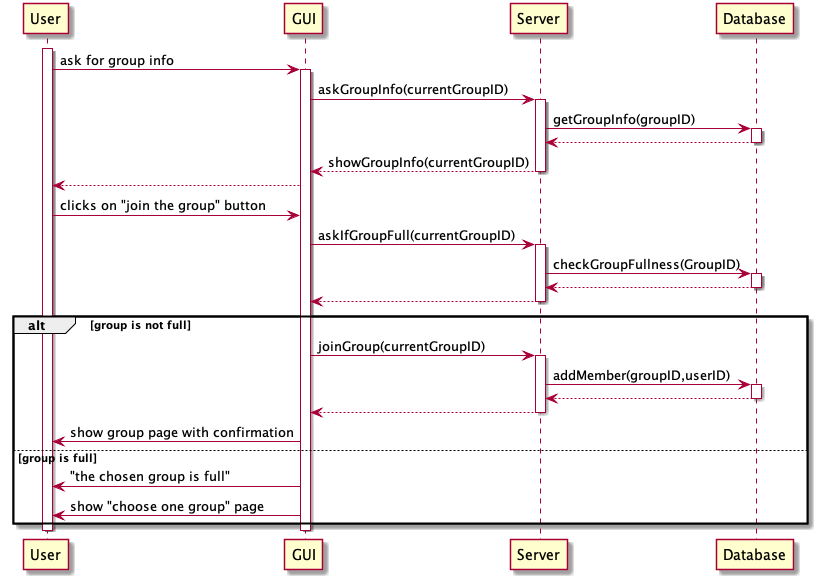
\includegraphics[width=0.93\textwidth]{Sequenzdiagramme/SD_checkInfo&joinGroup.png}
\end{center}

\subsection{Gruppe erstellen}
\begin{center}
	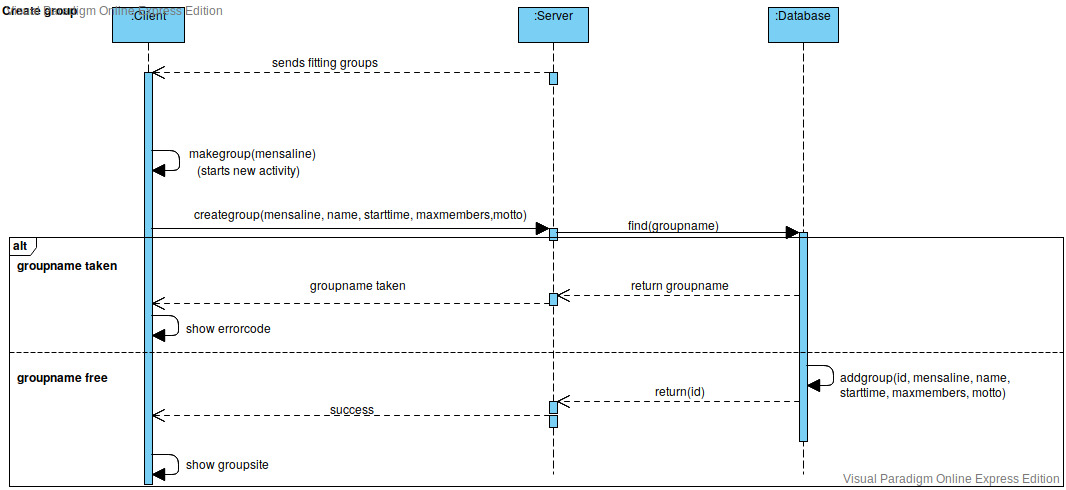
\includegraphics[width=0.93\textwidth]{Sequenzdiagramme/CreateGroup.jpg}
\end{center}

\subsection{Gruppe verlassen}
\begin{center}
	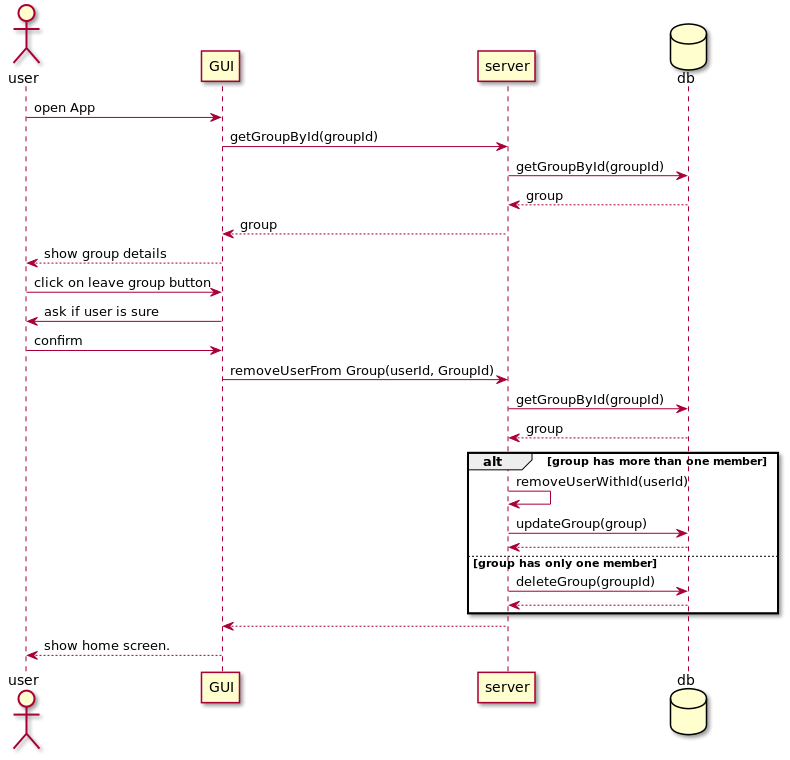
\includegraphics[width=0.93\textwidth]{Sequenzdiagramme/leaveGroupSD.png}
\end{center}


\chapter{Änderungen zum Pflichtenheft}

\chapter{Glossar}

\chapter{Anhang}

\end{document}
